\chapter{Knacken von MD5 mit OpenCL}
\rhead{Knacken von MD5 mit OpenCL}
\begin{refsection}

\chapterauthor{Danilo Bargen, Lukas Murer}

\section{Einleitung}

%- Was ist ein Hash-Algorithmus?
%- Was ist MD5?
%- Was ist Brute Force Cracking?
%- "Uberlegungen zum Keyspace
%- Zielsetzung

\subsection{Hashfunktionen}
\index{Hashfunktion}

Hashfunktionen (zu Deutsch \textit{Streuwertfunktionen}) sind in der Informatik
allgegenw"artig. Die Aufgabe einer Hashfunktion ist es, eine beliebig grosse
Eingabemenge auf eine kleine Ausgabemenge mit fester L"ange abzubilden.
Anwendungsgebiete sind beispielsweise die Integrit"atspr"ufung von Daten
(Pr"ufsummen) oder das Verschleiern von Passw"ortern (Passwort-Hashes).

Mathematisch gesehen ist eine Abbildung $h: K \rightarrow S$ eine Hashfunktion,
wenn $|K| \geq |S|$ gilt. Dabei ist $K$ die Menge der Schl"ussel und $S$ die
Menge der m"oglichen Hashwerte.

Eine der einfachsten Hashfunktionen ist die Quersumme, bei welcher die
Ziffernwerte einer Zahl summiert werden.
\[
	q(1337) = 1 + 3 + 3 + 7 = 14
\]
Weitere bekannte Hashfunktionen sind die Divisions-Rest-Methode
(Modulo-Arithmetik), CRC-Pr"ufsummen (Integrit"atspr"ufung) oder der Secure Hash
Algorithm (Kryptologie).

Die Anforderungen an eine ``gute'' Hashfunktion sind Abh"angig vom
Anwendungsbereich. Bei der ISBN-10 ist beispielsweise lediglich eine
Plausibilit"atspr"ufung in Form einer Pr"ufsumme n"otig. Bei Anwendungsf"allen
in der Kryptologie (zum Beispiel beim Hashen von Passw"ortern) sind jedoch viele
weitere Kriterien relevant. Nachfolgend werden einige davon vorgestellt.

\subsection{Eigenschaften von Hashfunktionen}

\subsubsection{Chaos}

Die Ausgabe einer chaotischen Hashfunktion sollte f"ur "ahnliche Eingabewerte
v"ollig unterschiedlich sein. Eine kleine "Anderung am Eingabewert sollte eine
grosse "Anderung im Ausgabewert zur Folge haben.

\subsubsection{Schwierige Umkehrbarkeit}

Eine schwierig umkehrbare Hashfunktion hat zum Ziel die Berechnung des
Funktionswertes m"oglichst zu vereinfachen, aber die Umkehrung dieses Ergebnisses
(berechnen des Ausgangswertes aus der Abbildung) m"oglichst zu erschweren. Anders
gesagt, es soll praktisch nicht m"oglich sein, zu einem gegebenen Hashwert $x$
eine Nachricht $m$ zu finden, f"ur welche $h(m) = x$ gilt.  Funktionen welche
diese Eigenschaft erf"ullen werden auch Einwegfunktionen genannt.

\subsubsection{Surjektivit"at}

Bei einer surjektiven Hashfunktion ist kein Ausgabewert unm"oglich, jeder kann
tats"achlich vorkommen.

\subsubsection{Kollisionsresistenz}
\label{crypto:kollisionsresistenz}
\index{Kollisionsresistenz}

Eine Kollisionsresistente Hashfunktion sollte es erschweren, zwei Eingabewerte
zu finden die den selben Ausgabewert ergeben. Daf"ur sollten die Ausgabewerte
m"oglichst gleichverteilt auftreten.

In der Kryptologie wird zwischen schwacher und starker Kollisionsresistenz
unterschieden\cite{crypto:stephan2011kryptographie}:

\begin{itemize}
		\item Schwache Kollisionsresistenz heisst, dass es praktisch nicht m"oglich
			ist, zu einer gegebenen Nachricht $m_0$ eine zweite Nachricht $m_1$ zu finden, f"ur
			welche $h(m_0) = h(m_1)$ gilt.
		\item Starke Kollisionsresistenz heisst, dass es praktisch nicht m"oglich
			ist, zwei Nachrichten $m_0$ und $m_1$ zu finden, f"ur welche $h(m_0) =
			h(m_1)$ gilt.
\end{itemize}

\subsubsection{Effizienz}

Je nach Anwendungsfall m"ochte man effiziente oder ineffiziente Berechnungen
eines Hashwertes erzielen. W"ahrend ersteres logisch erscheint -- man m"ochte
den Algorithmus in Hard- und Software m"oglichst einfach und schnell
implementieren k"onnen -- ist letzteres auf den ersten Blick ein merkw"Urdiges
Ziel. Die Eigenschaft ist jedoch vor allem f"ur Passwort-Hash-Funktionen
relevant. Um zu verhindern dass ein Angreifer m"oglichst schnell alle m"oglichen
Passw"orter vorberechnet, m"ochte man eine Funktion welche aufw"andig und
ressourcenintensiv zu berechnen ist.

\subsection{MD5}
\index{MD5}

Der MD5 Algorithmus (Message-Digest Algorithm 5) wurde im Jahr 1991 vom
Kryptologen Ronald L. Rivest entwickelt. MD5 erzeugt zu einer beliebigen
Nachricht einen 128-Bit Hashwert.

Unter Unix-basierten Betriebssystemen kann man MD5-Werte ganz einfach auf der
Kommandozeile berechnen:

\begin{verbatim}
$ echo -n "Mathematisches Seminar" | md5sum 
47b2d986d0ae09d6504b9696e9406ca4
\end{verbatim}

Man sieht also, dass der Eingabewert ``Mathematisches Seminar'' auf den
Ausgabewert \texttt{47b2\-d986\-d0ae\-09d6\-504b\-9696\-e940\-6ca4} (in
hexadezimaler Notation) abgebildet wird. Wenn man nun nur ein einzelnes
Zeichen im Eingabestring "andert, sieht die Ausgabe v"ollig anders aus
($\rightarrow$ Chaoseigenschaft):

\begin{verbatim}
$ echo -n "Mathematisches Saminar" | md5sum 
625a5fb1280f153aa06709d70b38dfb8
\end{verbatim}

MD5 war (und ist) weit verbreitet und wurde in der Vergangenheit neben der
Integrit"atspr"ufung auch h"aufig zum Verschleiern von Passw"ortern verwendet.
Wie dies funktioniert, l"asst sich einfach an einem Praxisbeispiel
demonstrieren:

\begin{enumerate}
		\item Ein Benutzer registriert sich mit Benutzername und Passwort auf einer
			Website. Beide Werte werden an den Webserver "ubertragen.
		\item Der Server berechnet den Hashwert des Passwortes. Das Passwort wird
			verworfen, nur der Hashwert wird gespeichert.
		\item Der User m"ochte sich zu einem sp"ateren Zeitpunkt wieder einloggen.
			Daf"ur "ubermittelt er erneut das Passwort an den Server.
		\item Der Server berechnet erneut den Hashwert des Passwortes und
			vergleicht diesen mit dem zuvor gespeicherten Wert. Stimmen die beiden
			Werte "uberein, wird dem Benutzer Zugang zu den gesch"utzten Inhalten
			gew"ahrt.
\end{enumerate}

An diesem Beispiel erkennt man auch sehr gut, wie wichtig die Einwegeigenschaft
und die Kollisionsresistenz f"ur kryptologische Hashfunktionen ist. Sollte
n"amlich ein Passwort-Hash an die "Offentlichkeit gelangen (beispielsweise durch
ein Datenleck, wie sie in den letzten Jahren -- zuletzt bei Adobe -- immer
wieder geschehen sind), sollte es f"ur einen Angreifer mit praktischem Aufwand
nicht m"oglich sein, ausgehend vom Hashwert das urspr"ungliche Passwort zu
errechnen. Ebensowenig sollte es m"oglich sein, ein anderes Passwort zu finden
welches den selben Hashwert ergibt. In beiden F"allen w"are das Benutzerpasswort
dadurch kompromittiert.

MD5 gilt inzwischen als unsicher, weil erfolgreiche Angriffe auf die
Kollisionsresistenz des Algorithmus gefunden wurden. Bereits im Jahr 2006 gelang
es Forschern, MD5-Kollisionen auf einem Pentium 4 Rechner im Durchschnitt
innerhalb einer Minute zu finden\cite{crypto:stevens2006fast}. Inzwischen sind
Kollisionen auf markt"ublicher Hardware innerhalb weniger Sekunden berechenbar.
Der MD5-Algorithmus ist also h"ochstens schwach kollisionsresistent
(\ref{crypto:kollisionsresistenz}) und sollte f"ur kryptologische Anwendungen
nicht mehr eingesetzt werden.

\subsection{Brute-Force Angriff auf MD5}
\index{Brute-Force}

W"ahrend Kollisionen f"ur frei gew"ahlte Eingabewerte wie im letzten Abschnitt
beschrieben heute problemlos berechenbar sind, ist bisher noch kein praktischer
Preimage-Angriff auf MD5 bekannt. Ein Preimage-Angriff bedeutet, dass der
Ausgabewert nicht frei gew"ahlt werden kann, sondern festgelegt ist (ein Angriff
auf die schwache Kollisionsresistenz). Wenn man nun einen Passwort-Hash
zur"uckrechnen will, ist bei einer "uberschaubaren Eingabemenge ein Brute-Force
Angriff die einfachste M"oglichkeit.

Bei einem Brute Force Angriff wird f"ur jeden Wert einer bestimmten
Eingabemenge der Hash\-wert berechnet und mit dem Zielwert verglichen. In
Pseudocode:

\begin{verbatim}
target = "47b2d986d0ae09d6504b9696e9406ca4"
for word in keyspace:
  if md5(word) == target:
    print(word)
    break
\end{verbatim}

\label{crypto:keyspace}
\index{Keyspace}
Die Eingabemenge nennt man auch ``Keyspace''. Will man beispielsweise f"ur alle
Passw"orter bestehend aus den Klein- und Grossbuchstaben a-z / A-Z sowie den
Zahlen 0-9 mit einer L"ange von bis zu 6 Zeichen die Hashes berechnen, ergibt
dies "uber 57 Milliarden M"oglichkeiten.
\[
	\sum_{i=1}^{6} \left(26 + 26 + 10\right)^i = 57'731'386'986
\]
Hier sieht man auch schon die Schwierigkeit an der Sache, denn der Keyspace
w"achst exponentiell. Bei Erh"ohung der Maximall"ange auf 8 Zeichen sind wir schon
in der Gr"ossenordnung von ~200 Billionen.
\[
	\sum_{i=1}^{8} \left(26 + 26 + 10\right)^i = 221'919'451'578'090
\]
Im Rahmen dieser Arbeit beschr"ankten wir daher sowohl die Anzahl der m"oglichen
Zeichen wie auch die maximale L"ange der zu knackenden Passw"orter.

% TODO danilo: ev eine line-grafik?

\subsection{Zielsetzung}
\label{crypto:zielsetzung}

Unser Ziel im Rahmen dieser Arbeit war es, durch massiv parallele Berechnung von
MD5-Hashwerten dasjenige Eingabewort zu finden, dessen MD5-Hashwert einem zuvor
festgelegten Hashwert entspricht. Der Keyspace besteht dabei aus den
Kleinbuchstaben a-z mit einer variablen L"ange von bis zu 6 Zeichen.

Konkret haben wir uns als Ziel gesetzt in m"oglichst kurzer Zeit den MD5-Hash
des Wortes ``monkey'' (Platz 6 auf der Liste der am h"aufigsten verwendeten
Passw"orter 2012 \cite{crypto:splash2012}) zu knacken.

\begin{verbatim}
$ echo -n "monkey" | md5sum
d0763edaa9d9bd2a9516280e9044d885
\end{verbatim}

\section{Umsetzung mit OpenCL}

Wenn man einen MD5-Hash brute-forcen will, ben"otigt man eine massive Anzahl
komplett unabh"angiger paralleler Tasks. Die MD5-Berechnung selbst ist nicht
unabh"angig und wird deshalb nicht parallelisiert, aber mehrere MD5-Berechnungen
k"onnen nebeneinander ausgef"uhrt werden und ben"otigen keinerlei
Interprozess-Kommunikation. OpenCL ist hierf"ur also bestens geeignet.

\section{Probleme mit grossen Problemen}
\label{crypto:grosse_probleme}

\subsection{Einf"uhrung}

Auch wenn OpenCL ausdr"ucklich daf"ur entwickelt wurde, mit riesigen Clustern
von heterogenen Recheneinheiten sehr umfangreiche Probleme zu l"osen, so st"osst
man doch irgendwann an die Grenzen der Hardware oder der Implementierung.  Denn
jeder Kernel der ausgef"uhrt wird, ben"otigt Speicherplatz (Gr"osse des zur
Verf"ugung stehenden Speichers, Hardware) und muss irgendwie verwaltet werden
(Anzahl der maximal verwaltbaren Work-Items und Work-Groups, Implementierung).
Zudem ist die Anzahl Dimensionen, die von einem Kernel verarbeitet werden kann,
begrenzt (Work-Item-Dimension, Hardware \& Implementierung). Deshalb folgen in
diesem Kapitel einige Betrachtungen dazu, wie man mit diesen Limitationen
umgehen kann.

% TODO: Im Kapitel "Brute-Force Angriff auf MD5" werden fast die selben
% Berechnungen (Kombinatorik) bereits gemacht. Ev kann man darauf verweisen,
% anstatt sie hier nochmals zu machen?
Angenommen wir verwenden nur den Zeichensatz [a-zA-Z0-9] sprich insgesamt 62 
unterschiedliche Zeichen, die beliebig kombiniert werden k"onnen. Die 
Kombinatorik sagt dazu, dass es also

\[
 N_{Komb} =  62^{n}
\]

m"ogliche Kombinationen gibt,  wobei \[n\] die Anzahl der Zeichen im Wort angibt. 
Das ergibt bei einer Stellenzahl von 8 Stellen, was so in etwa der gel"aufigen 
Mindestl"ange eines Passworts entspricht 

\[ 
 N_{Komb} = 62^{8} = 2.183 * 10^12 
\] 

Kombinationen. Demgegen"ber stehen aber auf einem System mit einem Intel i5-3320M 
Prozessor und 8GB RAM und in einer OpenCL Workgroup maximal

\[
 N_{max} = N_{Workitems}^{wi_dim} = 8193^{3} = 5.50 * 10^11
\]

verwaltbare ``Problem-St"ucke'' entgegen. Trotzdem l"asst zum Beispiel die OpenCL
Implementierung von Intel auch eine gr"ossere Anzahl WorkItems problemlos zu, 
wohingegen sich die Nvidia Implementation mit einer ``Out-of-resources''-Meldung 
beendet.

Genau um diese Grenzen soll es in diesem Abschnitt gehen. Es soll aber in keinster
Weise ersch"opfend die Grenzen von OpenCL oder alle Spezifikas der 
Implementierungen eingegangen werden, sondern vielmehr f"ur das Thema sensibilisiert 
und m"ogliche Ans"atze f"ur den Umgang mit grossen Problemen in OpenCL aufgezeigt
werden, was hoffentlich dazu f"uhren wird, dass der Leser/die Leserin ein Gesp"ur 
f"ur eigene, auf die spezifische Hardware und Implementierung zugeschnittene 
Ans"atze entwickeln kann.


\subsection{Grenzen von OpenCL}

% TODO: Ich würde auf Erweiterungen gar nicht erst eingehen. Sie sind für uns ja
% nicht sonderlich relevant.
OpenCL wurde entwickelt um trotz einem m"glichst Plattform"ubergreifenden Ansatz 
sehr flexibel auf die Spezifika der jeweiligen Hardware reagieren zu k"onnen, was
auch das ebenfalls in OpenGL vorhandene Extension-System beinhaltet. Vor allem f"ur
% TODO: Hier ebenfalls, ich würde OpenGL gar nicht erst erwähnen, sondern ganz
% auf OpenCL fokussieren.
Einsteiger in die OpenCL/OpenGL-Welt (hier sei erw"ahnt, dass hinter beiden 
Technologien sehr "anhliche Grundkonzepte stehen) kann es dabei schwierig werden
sich im Dschungel der Hardwaredaten und M"oglichkeiten zurechtzufinden. Auf die 
wichtigsten Einstiegspunkte und die f"ur unsere Problemstellung relevanten Punkte
soll hier kurz eingegangen werden.


\subsubsection{Hardwaremerkmale abfragen}

Gerade weil OpenCL so unterschiedliche Typen Hardware unterst"utzt, von der ``normalen''
Desktop-CPU bis zu f"ur HPC Anwendungen spezialisierte Rechenkarten, gibt es einen
sehr m"achtigen Weg die jeweiligen Hardwaremerkmale abzufragen. Das kann soweit 
gehen, dass w"ahrend der Laufzeit die Hardwarekonfiguration abgefragt und das 
Problem dynamisch auf die vorhandene Hardware optimiert wird.

An dieser Stelle macht es Sinn sich nochmals vereinfacht die Top-Down-Struktur
von OpenCL (wie bereits in Abbildung \ref{hardware:opencl} gezeigt) vor Augen zu
f"uhren: \texttt{Platform $\rightarrow$ Compute Device $\rightarrow$ Compute
	Unit ($\rightarrow$ Work Group $\rightarrow$ Work Item $\rightarrow$ Work Item
Dimension)}. In dieser Reihenfolge werden auch die Hardwaremerkmale abgefragt.
OpenCL 1.2 stellt dazu folgende Funktionen zur Verf"ugung:

\begin{description}
 \item [clGetPlatformIDs()] gibt eine Liste der vorhandenen Plattformen zur"uck.
 \item [clGetPlatformInfo()] retourniert die Merkmale der aktuellen Plattform. Das heisst,
                            der Herausgeber der Implementation, die imlementierte 
                            OpenCL Version und allf"allig von der Plattform 
                            zus"atzlich unterst"utzte Erweiterungen (Das m"ussen
                            nicht die gleichen sein wie die von den jeweiligen
                            Compute Devices unterst"utzten).
 \item [clGetDeviceIDs()]   Mit der jeweiligen Plattform-ID k"onnen nun die auf der 
                            jeweiligen Plattform verf"ugbaren Compute-Devices abgefragt 
                            werden.
 \item [clGetDeviceInfo()]  Mit den so erhaltenen Device-IDs bekommt man anschliessend 
                            zum abgefragten Compute Device einen ganzen Katalog von
                            Merkmalen zur"uck, von der maximalen Anzahl von Workgroups
                            und Work-Items, "uber die Speicherkapazit"aten bis zur 
                            Clock-Frequenz und dem Hersteller der Hardware. Auf einzelne 
                            dieser Merkmale soll im Folgenden noch eingegangen werden.
\end{description}

\noindent Die genauen Parameter und R"uckgabewerte k"onnen der offiziellen
Dokumentation \cite{crypto:opencl_ref} entnommen werden.

Um das diese Begriffe etwas verst"andlicher zu machen, wird ein kurzes
Code-Beispiel f"ur einen typischen Desktop-Computer mit einer OpenCL f"ahigen
CPU und einer modernen Grafikkarte aufgef"uhrt. Es ist exemplarisch, der
Anschaulichkeit wegen in Pseudocode verfasst und repr"asentiert weder den vollen
Umfang der R"uckgabewerte noch die real ben"otigten Parameter!

\begin{small}
\begin{verbatim}
> clGetPlatformIDs()
0
1

> clGetPlatformInfo(platform=0)
Name:          Intel(R) OpenCL
Vendor:        Intel(R) Corporation
Version:       1.2
Profile:       Full
Extensions:    cl_khr_icd,cl_khr_global_int32_base_atomics,(...)

> clGetPlatformInfo(platform=1)
Name:          NVIDIA(R) OpenCL
Vendor:        NVIDIA Corp. limited
Version:       1.2
Profile:       Full
Extensions:    (...)

> clGetDeviceIDs(platform=0)
0

> clGetDeviceInfo(platform=0,device=0)
General Information:
 - Name:                 Intel(R) Core(TM) i5-3320M CPU @ 2.60GHz
 - Available:            True
 - Vendor (VID):         Intel(R) Corporation (32902)
 - Version:              OpenCL 1.2 (Build 82248)
 - Profile:              full
 - Type:                 CPU 
 - Extensions:           cl_khr_icd,cl_khr_global_int32_base_atomics,(...)
 - Endianess:            Little

Memory and Clocks
 - Clock frequency (max):2600 MHz
 - Compute units:        4
 - Global memory:        7816 MB
 - Local memory:         32768 kB, 2

Kernel properties:
 - Max param. size:      3840 B
 - Max work group size:  8192
 - Max work item dim.:   3
 - Max work item size:   [8192, 8192, 8192]

Datatypes:
 - Flotating point:      Single & Double precision
 - Preferred vector size: 1 (all supported  types)
\end{verbatim}
\end{small}

\vspace{1em}

\noindent Zu einzelnen Punkten aus dem Codebeispiel hier eine kurze Erl"auterung:

\begin{description}
 \item [Version] Implementierte bzw. Unterst"utzte OpenCL Version
 \item [Profile] \texttt{full} oder \texttt{embedded} (in OpenCL 1.2)
 \item [Type]    \texttt{CPU}, \texttt{GPU} oder \texttt{ACCELERATOR}
 \item [Compute Units] Anzahl der physisch vorhandenen Compute Units. Dies ist
                 die Anzahl effektiv parallel ausgef"uhrter Kernel
 \item [Max work group size] Maximale Anzahl Work Items in einer Work Group
 % TODO: Stimmt das "minimal 3"? Sind das nicht maximal 3?
 \item [Max work item dim.] Maximale direkt im Work Item bearbeitbare Dimensionen, minimal 3
 \item [Max work item size] Maximale Anzahl von Work Items in einer Work Group nach
                 Dimensionen (Ist je nach Ger"at unterschiedlich je nach
                 Dimension)
 \item [Preferred vector size] (Nach Datentyp) Vektorgr"osse, die von der Hardware 
                 f"ur den jeweiligen Typ direkt (in einer Instruktion) verarbeitet
                 werden kann.
 
\end{description}


\noindent Dabei gelten anhand der im Code gezeigten Zahlen gem"ass
Spezifikation\cite{crypto:opencl_ref} folgende Regeln:

\begin{itemize}
 \item Eine Work Group wird nur auf einer Compute Unit aufgef"uhrt (1 Work Group = 1 
       Compute Device) 
 \item Die Anzahl der Work-Items pro Work-Group darf insgesamt 8192 nicht "ubersteigen (global work size)
 \item Dabei d"urfen die in ``Max work item size'' angegebenen Werte in der jeweiligen 
       Dimension nicht "uberstiegen werden (local work size $[x,y,z,\ldots]$).
			 Die Summe $x + y + z$ darf dabei aber nicht gr"osser werden als ``Max work group size''.
 \item Die Anzahl effektiv verwendeter Work Item Dimensionen darf im Bereich von 1 bis
       ``Max work item dim.'' liegen.
\end{itemize}


\subparagraph{Maximale Problemgr"osse an einem Beispiel}

Das heisst nun f"ur unser Beispiel folgendes:

\begin{itemize}
 \item asdg
\end{itemize}








- Wo stossen wir an unsere Grenzen?
- Bezug/Referenz auf Einleitung ("Uberlegungen zum Keyspace)

\subsection{Aufteilung von grossen Problemen}

- Was gibt es f"ur L"osungsans"atze?




\section{L"osungsansatz}

% TODO danilo: Ev Bezug auf vorherige Section

Um den Brute-Force-Knacker zu implementieren haben wir uns f"ur folgenden
L"osungsansatz entschieden:

\begin{itemize}
	\item Jedes m"ogliche Eingabewort (siehe "Uberlegungen zum Keyspace in Kapitel
		\ref{crypto:keyspace}) wird einem Kernel zugewiesen.
	\item Jeder Kernel berechnet den MD5-Hash f"ur genau ein Wort.
	\item Das Eingabewort wird innerhalb des Kernels aus der Global ID
		hergeleitet.
	\item Der errechnete Hash wird innerhalb des Kernels mit dem Ziel-Hash
		verglichen. Sofern die zwei Werte "ubereinstimmen, wird das Wort in den
		Result-Buffer geschrieben.
	\item Der Einfachheit halber wird im Erfolgsfall kein vorzeitiger Abbruch
		durchgef"uhrt, stattdessen wird der ganze Keyspace durchprobiert. Dies
		erm"oglicht auch einfache Performance-Vergleiche auf verschiedenen
		Plattformen.
	\item Nachdem alle m"oglichen Hash-Werte berechnet wurden, wird der
		Result-Buffer vom Hauptprogramm ausgelesen und angezeigt.
\end{itemize}

\noindent Zusammengefasst besteht der Ablauf aus drei Phasen: Init (CPU),
Calculate (GPU), Collect (CPU).

\begin{figure}[H]
	\centering
	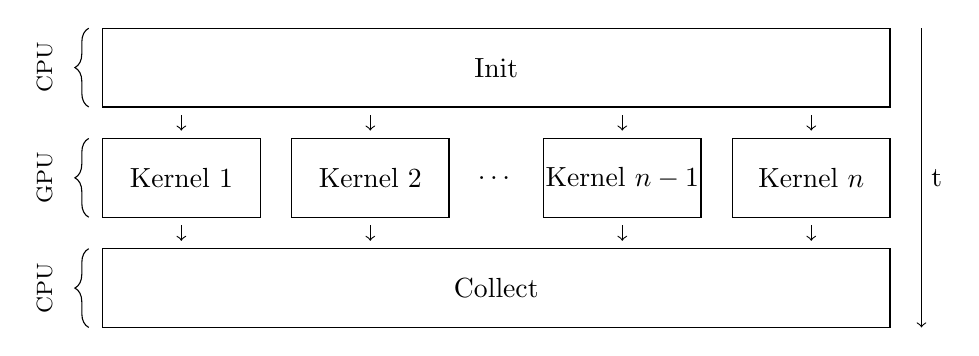
\begin{tikzpicture}

	% Init
	\draw (0,2.8) rectangle node {Init} (10,3.8);

	% Kernels
	\draw (0,1.4) rectangle node {Kernel $1$} (2,2.4);
	\draw (2.4,1.4) rectangle node {Kernel $2$} (4.4,2.4);
	\draw (5,1.9) node {\ldots};
	\draw (5.6,1.4) rectangle node {Kernel $n-1$} (7.6,2.4);
	\draw (8,1.4) rectangle node {Kernel $n$} (10,2.4);

	% Collect
	\draw (0,0) rectangle node {Collect} (10,1);

	% Time arrow
	\draw[<-] (10.4,0) -- node [right] {t} (10.4,3.8);

	% Flow arrows
	\foreach \x in {1, 3.4, 6.6, 9} {
		\draw[<-] (\x,1.1) -- (\x,1.3);
		\draw[<-] (\x,2.5) -- (\x,2.7);
	}

	% Curly braces
	\draw [decorate,decoration={brace,amplitude=5pt},xshift=-5pt]
		(0,2.8) -- (0,3.8) node[midway,xshift=-16pt,rotate=90] {\footnotesize CPU};
	\draw [decorate,decoration={brace,amplitude=5pt},xshift=-5pt]
		(0,1.4) -- (0,2.4) node[midway,xshift=-16pt,rotate=90] {\footnotesize GPU};
	\draw [decorate,decoration={brace,amplitude=5pt},xshift=-5pt]
		(0,0) -- (0,1) node[midway,xshift=-16pt,rotate=90] {\footnotesize CPU};

\end{tikzpicture}

	\caption{L"osungsansatz Programmstruktur}
	\label{img:crypto:programm-struktur}
\end{figure}

\subsection{Herleitung Wort aus Global ID}
\index{Global ID}

Irgendwie muss nun jeder Kernel herausfinden, welches Wort er hashen soll. Eine
"Ubergabe des zu hashenden Wortes vom Hauptprogramm an jeden Kernel via Shared
Memory w"are ineffizient und w"urde nur unn"otigen I/O verursachen. Es muss also
eine bessere L"osung gefunden werden.

Ein Vorteil des gegebenen Problemes ist, dass der Keyspace f"ur die m"oglichen
Eingabewerte einen Linearen Raum darstellt. Es liegt also nahe, das Wort aus der
Global ID herzuleiten. Die Global ID ist eine $n$-Dimensionale nat"urliche Zahl,
welche jedem Kernel von OpenCL zugewiesen wird. Der Wertebereich bewegt sich
dabei in Einerschritten von $(0, ..., 0)$ bis $(s_1, ..., s_n)$. Dabei ist $s_n$
die \textit{Work Size} f"ur die entsprechende Dimension $n$.

\subsubsection{Naiver Ansatz}

Ein naiver Ansatz w"are nun, dass die jede Dimension der Global ID einem
m"oglichen Zeichen des Eingabewortes entspricht. Die Dimensionszahl entspricht
dann der Anzahl Zeichen im Eingabewort. Um diesen Ansatz zu verdeutlichen,
nachfolgend ein Pseudocode-Beispiel f"ur ein Eingabewort mit der L"ange 3 und
dem Alphabet a-z:

\begin{small}
\begin{verbatim}
>>> id = (22, 19, 5)
>>> alphabet = "abcdefghijklmnopqrstuvwxyz"
>>> word = alphabet[id[0]] + alphabet[id[1]] + alphabet[id[2]]
>>> print(word)
wtf
\end{verbatim}
\end{small}

\noindent Das sieht zwar auf den ersten Blick nach einem guten Ansatz aus,
jedoch ergibt sich dabei das erste Problem: Die Anzahl Dimensionen der Global ID
(Work Size Dimension) darf gem"ass OpenCL Standard\cite{crypto:opencl_ref}
maximal 3 sein. Das bedeutet, dass man mit diesem Ansatz nur W"orter mit einer
L"ange von bis zu 3 Zeichen knacken kann. Man muss also einen Weg finden, diese
Dimensionen irgendwie zu vergr"ossern.

\subsubsection{Virtuelle Dimensionen}

Eine M"oglichkeit dazu ist die Einf"uhrung virtueller Dimensionen. Dabei werden
mehrere Dimensionen durch Multiplikation der Keyspace-Gr"osse in eine einzelne
``Virtuelle Dimension'' gepackt. Konkret sieht das so aus:

\begin{itemize}
	\item Dimension bei Wort-L"ange 1: $(26,)$
	\item Dimension bei Wort-L"ange 3: $(26, 26, 26)$
	\item Dimension bei Wort-L"ange 4: $(26^2, 26, 26) = (676, 26, 26)$
	\item Dimension bei Wort-L"ange 7: $(26^3, 26^2, 26^2) = (17576, 676, 676)$
\end{itemize}

\noindent Aus diesen Werten kann dann der Buchstabe $c_n$ an Position $n$ mithilfe von
Modulo-Arithmetik aus der jeweiligen Work Size $d$ abgeleitet werden:
\[
	c_n = \frac{d}{26^n} \mod\enskip 26
\]
Um nun den entsprechenden ASCII-Buchstaben zu erhalten, muss man lediglich
diesen Wert $c_n$ um 97 (ASCII-Position des Kleinbuchstabens \texttt{a})
erh"ohen.

Damit das Ganze etwas einfacher zu implementieren ist, f"uhren wir zus"atzlich
das Konzept eines ``Triplets'' ein. Die Triplet-ID ergibt sich, wenn man die
Buchstaben des Wortes in Dreiergruppen aufteilt (Sliding Window Algorithmus).

\begin{figure}[H]
	\centering
	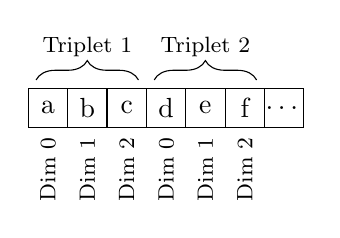
\begin{tikzpicture}

	% Rechtecke
	\draw (0,0) rectangle node {a} (0.5, 0.5);
	\draw (0.5,0) rectangle node {b} (1, 0.5);
	\draw (1,0) rectangle node {c} (1.5, 0.5);
	\draw (1.5,0) rectangle node {d} (2, 0.5);
	\draw (2,0) rectangle node {e} (2.5, 0.5);
	\draw (2.5,0) rectangle node {f} (3, 0.5);
	\draw (3,0) rectangle node {\ldots} (3.5, 0.5);

	% Labels unten
	\foreach \x in {0, 1.5} {
		\draw (\x+0.25,0) node[left,rotate=90] {\footnotesize Dim 0};
		\draw (\x+0.75,0) node[left,rotate=90] {\footnotesize Dim 1};
		\draw (\x+1.25,0) node[left,rotate=90] {\footnotesize Dim 2};
	}

	% Klammern
	\draw [decorate,decoration={brace,amplitude=7pt},xshift=0pt,yshift=3pt]
		(0.1,0.5) -- (1.4, 0.5) node[midway,yshift=12pt] {\footnotesize Triplet 1};
	\draw [decorate,decoration={brace,amplitude=7pt},xshift=0pt,yshift=3pt]
		(1.6,0.5) -- (2.9, 0.5) node[midway,yshift=12pt] {\footnotesize Triplet 2};

\end{tikzpicture}

	\caption{Aufteilung des Wortes in Triplets}
	\label{img:crypto:triplets}
\end{figure}

\noindent In OpenCL C sieht das folgendermassen aus:

\begin{small}
\begin{verbatim}
// Initialize private variables
__private char string[MAX_PW_LEN];
__private unsigned int global_id;
__private unsigned char triplet_id;

for (int i = 0; i < 3; i++) {

  // Get global ID for dimension i
  global_id = get_global_id(i);

  // Loop through triplets
  for (triplet_id = 0; triplet_id <= (len - 1) / 3; triplet_id += 1) {
    string[triplet_id * 3 + i] = 0x61 + ((int)(global_id / pown(26., triplet_id)) % 26);
  }

}
\end{verbatim}
\end{small}

\section{Implementationsdetails}

\subsection{Berechnung des MD5-Wertes}
\label{crypto:md5lib}

Zur effektiven Berechnung des MD5-Wertes haben wir eine bereits bestehende
C-Implementierung des MD5-Algorithmus
verwendet\footnote{\url{http://openwall.info/wiki/people/solar/software/public-domain-source-code/md5}},
welche im Jahr 2001 von \textit{RSA Data Security, Inc.} geschrieben und dann
als gemeinfrei ver"offentlich wurde.

Die Library musste geringf"ugig angepasst werden, um innerhalb eines OpenCL
Kernels lauff"ahig zu sein. Beispielsweise mussten alle dynamischen
Memory-Manipulationen wie \texttt{memcpy} und \texttt{memset} durch
entsprechende statischen Loops ersetzt werden, da OpenCL keine dynamische
Memory-Al\-lo\-ka\-ti\-on erlaubt. Auch mussten Address Space Qualifier (wie
\texttt{\_\_constant}, \texttt{\_\_private}, etc) erg"anzt werden.

Nach erfolgten Anpassungen kann ein MD5-Hash innerhalb des OpenCL Kernels
folgendermassen errechnet werden:

\begin{small}
\begin{verbatim}
__private MD5_CTX context;
__constant unsigned char len;
__private char string[MAX_PW_LEN];
__private unsigned char digest[16];

MD5_Init(&context);
MD5_Update(&context, (const void *)string, len);
MD5_Final(digest, &context);
\end{verbatim}
\end{small}

\subsection{Verifikation des Resultates}
\label{crypto:verifikation}

In jedem Kernel wird der berechnete MD5-Hash mit dem Ziel-Hash verglichen.
Stimmen sie "uberein, so wird das verwendete Eingabewort in den Result-Buffer im
Global Memory geschrieben.

\begin{small}
\begin{verbatim}
// Copy matching string from private to global memory
if (compare(hash, digest, 16) == 0) {
  for (int i = 0; i < len; i++) {
    result[i] = string[i];
  }
}
\end{verbatim}
\end{small}

\subsection{Init \& Collect}

\subsubsection{Init}

Die Aufgabe der Initialisierungsphase ist es, das gew"unschte OpenCL Device
auszuw"ahlen, die Kernel zu konfigurieren und zu initialisieren und dann zu
starten.

Wir haben im Rahmen dieser Arbeit nicht direkt mit den OpenCL C Libraries
gearbeitet, sondern eine Wrapper-Library namens
PyOpenCL\footnote{\url{http://documen.tician.de/pyopencl/}} f"ur die
Programmiersprache Python\footnote{\url{https://www.python.org/}} verwendet. Im
direkten Vergleich mit C ist es so viel einfacher OpenCL zu initialisieren und
zu konfigurieren (wobei nat"urlich Python-Kenntnisse n"otig sind). Auf die
Syntax von Python und die Implementations-Details der Library wird hier nicht
n"aher eingegangen.

Als Erstes muss ein OpenCL-Kontext und eine Command Queue eingerichtet werden:

\begin{small}
\begin{verbatim}
ctx = cl.create_some_context()
queue = cl.CommandQueue(ctx)
\end{verbatim}
\end{small}

\noindent Danach muss man die ganzen Buffer- und Result-Objekte vorbereiten:

\begin{small}
\begin{verbatim}
result = bytearray(MAX_PW_LEN)
result_string = bytearray(MAX_PW_LEN)

mf = cl.mem_flags
hash_buf = cl.Buffer(ctx, mf.READ_ONLY | mf.COPY_HOST_PTR, hostbuf=input_hash)
result_buf = cl.Buffer(ctx, mf.WRITE_ONLY | mf.COPY_HOST_PTR, hostbuf=result)
\end{verbatim}
\end{small}

\noindent Anschliessend wird der Kernel-Code aus der Datei \texttt{md5.cl}
geladen.

\begin{small}
\begin{verbatim}
with open('md5.cl', 'r') as f:
    fstr = ''.join(f.readlines())
    prg = cl.Program(ctx, fstr).build()
\end{verbatim}
\end{small}

\noindent Nun werden in $n$ Runden jeweils alle m"oglichen Eingabeworte der
L"ange $i$ berechnet, wobei $n$ der Maximall"ange des Eingabewortes entspricht
und $i$ die jeweilige Wortl"ange zwischen 1 und $n$ ist.

\begin{small}
\begin{verbatim}
for i in range(1, MAX_PW_LEN + 1):

    # Define work sizes
    global_worksize = []
    for j in range(i):
        if j < 3:
            global_worksize.append(ALPHABET_SIZE)
        else:
            global_worksize[j % 3] *= ALPHABET_SIZE
    local_worksize = None  # Let OpenCL figure out the best value

    # Run kernel!
    prg.crack(queue, global_worksize, local_worksize, hash_buf, result_buf, np.int8(i))

    # Copy result back to device
    cl.enqueue_read_buffer(queue, result_buf, result_string).wait()
\end{verbatim}
\end{small}

\noindent Der gesamte Code (inkl. aller Variablen- und Konstantendefinitionen
sowie aller Imports und Debug-Output) findet sich im Github-Repository (TODO URL
TO REPO).

\subsubsection{Collect}

In der Collection-Phase werden die Ergebnisse der Kernel entgegengenommen und
verarbeitet. Da das korrekte Resultat im Erfolgsfall immer in den Result-Buffer
geschrieben wird (vgl. Kapitel \ref{crypto:verifikation}), muss nun lediglich
dieser Buffer ausgelesen werden. Da Python nicht mit null-terminierten
Bytestrings sondern mit Unicode-Objekten arbeitet, m"ussen in unserem Fall
zus"atzlich noch diese Null-Bytes entfernt werden.

\begin{small}
\begin{verbatim}
# Strip null bytes, convert to unicode
plaintext = result_string.strip(b'\x00').decode('ascii')
if plaintext:
    print('Result is "%s"!' % plaintext)
else:
    print('Did not find a result.')
\end{verbatim}
\end{small}


\subsection{Limitationen der gew"ahlten L"osung}

\subsubsection{Ressourcen-Limits}
\label{crypto:resourcenlimits}

Abh"angig von der gew"ahlten Platform st"osst man mit diesem L"osungsansatz
relativ schnell an Ressourcen-Limits. Mit einer Nvidia GeForce GTX 760
Grafikkarte war bereits ab einer L"ange von 7 Zeichen Schluss:

\begin{small}
\begin{verbatim}
(...)
Starting round with length 7...
Work size: [17576, 676, 676]
Traceback (most recent call last):
  File "crack_md5.py", line 58, in <module>
    cl.enqueue_read_buffer(queue, result_buf, result_string).wait()
  File "/usr/lib/python3.4/site-packages/pyopencl/__init__.py", line 860, in new_func
    return func(*args, **kwargs)
pyopencl.RuntimeError: clEnqueueReadBuffer failed: out of resources
\end{verbatim}
\end{small}

Wir haben nicht genauer nachverfolgt ob diese Fehlermeldung durch einen Fehler
in der Library-Implementation verursacht wurde oder ob ein effektives
Hardware-Limit erreicht wurde, aber es ist offensichtlich dass man nicht
beliebig viele Kernel parallel laufen lassen kann (vgl. Kapitel
\ref{crypto:grosse_probleme}).

Ein m"oglicher L"osungsansatz w"are das Einf"uhren von Kernel-Gruppen mit einer
fixen Anzahl parallel ausf"uhrbarer Kernel. Diese Zahl k"onnte dann jeweils an
die verwendete Hardware angepasst werden. Die optimale Wahl dieses Parameters
k"onnte durch algorithmische Optimierungsverfahren (optionale ``Kalibrierung''
zu Beginn des Programms) automatisiert in Erfahrung gebracht werden.

\subsubsection{Vorzeitiger Abbruch}

Aktuell wird die Ausf"uhrung des Programms nicht vorzeitig abgebrochen, wenn ein
Kernel das Resultat gefunden hat. Dies w"are allerdings mit einem \textit{Result
Found} Flag, welches durch den erfolgreichen Thread im Globalen Memory gesetzt
wird, relativ einfach implementierbar. Jeder Kernel m"usste zu Beginn der
Ausf"uhrung dieses Flag "uberpr"ufen. Ist es gesetzt, wird die MD5-Berechnung im
Kernel gar nicht erst ausgef"uhrt. Zu bestimmten Zeitpunkten im Programm-Ablauf
(zB nach Beendigung einer Kernel-Gruppe gem"ass Kapitel
\ref{crypto:resourcenlimits}) k"onnte auch das Hauptprogramm dieses Flag
"uberpr"ufen und im Erfolgsfall das Erzeugen neuer Kernel abbrechen.

Da das korrekte Resultat durchschnittlich nach 50\% der Versuche gefunden wird
(vorausgesetzt nat"urlich dass sich die korrekte L"osung im Keyspace befindet),
w"urde ein vorzeitiger Abbruch die Programm-Laufzeit (abz"uglich des dadurch
eingef"uhrten Overheads) im Schnitt halbieren.

\subsubsection{Performance-Einbussen durch Python}

Die Wahl der Programmiersprache Python zur Implementierung des Hauptprogramms
verursacht nat"urlich leicht h"ohere Laufzeit w"ahrend der Init- und
Collection-Phase, da Python eine interpretierte High-Level Programmiersprache
mit Garbage-Collection ist. Da jedoch sowohl die PyOpenCL Library wie auch der
Kernel-Code in C geschrieben sind, sind diese Performance-Einbussen in der Regel
vernachl"assigbar, solange der Hauptteil der Arbeit im Kernel-Code geschieht.

\subsubsection{Optimierung der MD5-Implementation}

Wie schon im Kapitel \ref{crypto:md5lib} beschrieben, haben wir innerhalb
unseres Kernels eine bestehende MD5-Implementation verwendet. Diese
Implementation wurde mit dem Fokus auf Einfachheit entwickelt und nicht im
Hinblick auf maximale Performance. Im Rahmen dieser Arbeit haben wir keinerlei
Optimierungen innerhalb dieser Library vorgenommen. Eine Parallelisierung des
Algorithmus ist zwar aufgrund der rundenbasierten Natur von MD5 nicht m"oglich,
jedoch bietet die Implementation selbst viel Raum f"ur
Performance-Optimierungen. Wie gross die Welt der m"oglichen
OpenCL-Kerneloptimierungen ist, sieht man beispielsweise eindr"ucklich im
\citetitle{crypto:nvidia_bestpractices} \cite{crypto:nvidia_bestpractices}.


\section{Resultate}

Unsere Implementation kann das gesetzte Ziel aus Kapitel
\ref{crypto:zielsetzung} -- das Knacken des Wortes ``monkey'' innerhalb
m"oglichst kurzer Zeit -- erreichen:

\begin{small}
\begin{verbatim}
$ echo -n "monkey" | md5sum
d0763edaa9d9bd2a9516280e9044d885
$ python crack_md5.py d0763edaa9d9bd2a9516280e9044d885
Starting round with length 1...
Work size: [26]
Starting round with length 2...
Work size: [26, 26]
Starting round with length 3...
Work size: [26, 26, 26]
Starting round with length 4...
Work size: [676, 26, 26]
Starting round with length 5...
Work size: [676, 676, 26]
Starting round with length 6...
Work size: [676, 676, 676]
Result is "monkey"!

Stats
-----

- Elapsed total time: 1.204507s
- Length 1: Finished in 0.000510s
- Length 2: Finished in 0.000458s
- Length 3: Finished in 0.000330s
- Length 4: Finished in 0.002104s
- Length 5: Finished in 0.049636s
- Length 6: Finished in 1.151242s
- Length 7: Projected time would be 29.932286s
- Length 8: Projected time would be 778.239443s
- Keyspace: 308915776
\end{verbatim}
\end{small}

Man sieht also, dass unser Programm auf einer Nvidia GeForce GTX 760 Grafikkarte
den Keyspace von 308'915'776 m"oglichen Eingabeworten innerhalb von 1.15s
durchsuchen kann.

Bei den anschliessend ausgegebenen Laufzeiten (sowohl effektiv wie auch
extrapoliert) sieht man sehr gut die in Kapitel \ref{crypto:keyspace}
vorhergesagte exponentielle Entwicklung:

\begin{figure}[H]
	\centering
	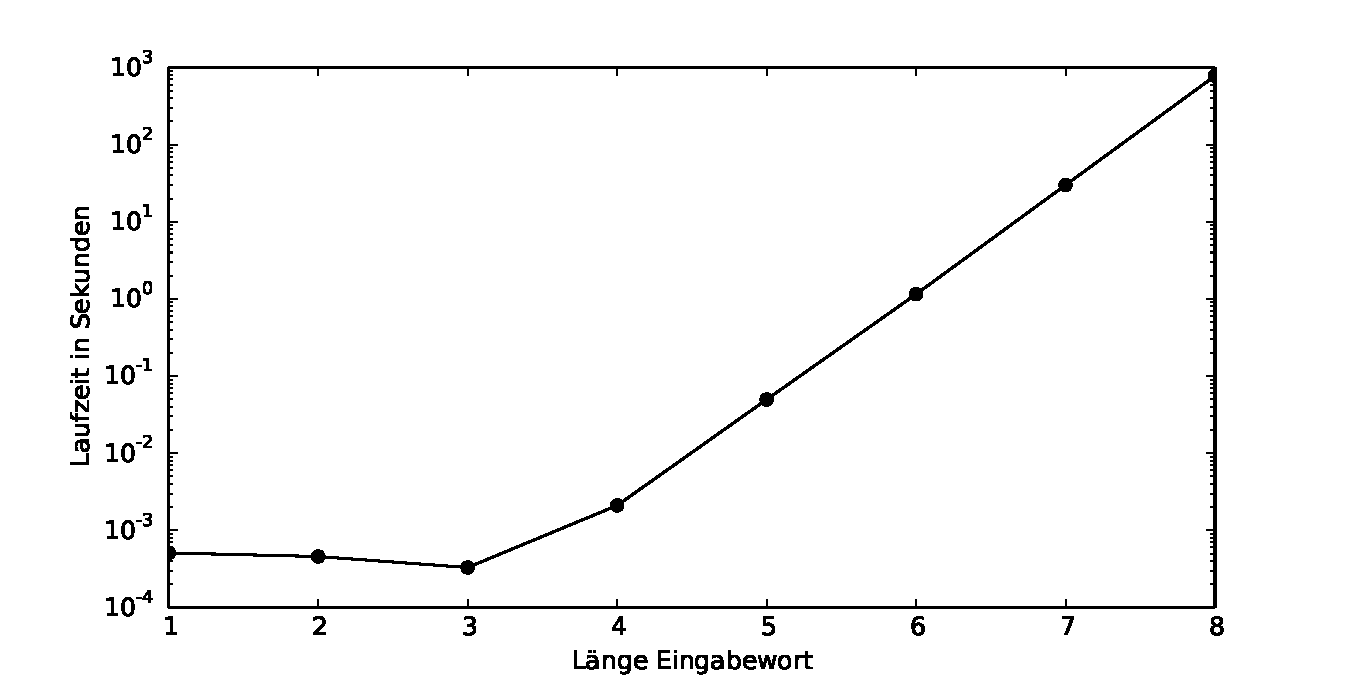
\includegraphics[width=.9\textwidth]{crypto/graphs/runtime.pdf}
	\caption{Entwicklung der Laufzeit abh"angig von der Wortl"ange}
	\label{img:crypto:triplets}
\end{figure}

\subsection{Performancevergleich}

Wir haben unsere Implementation auf verschiedenen CPU- und GPU-Platformen
getestet. Nachfolgend ein Vergleich der Laufzeit (tiefer ist besser) auf 3 CPUs
(Blau) und 3 GPUs (Gr"un):

\begin{figure}[H]
	\centering
	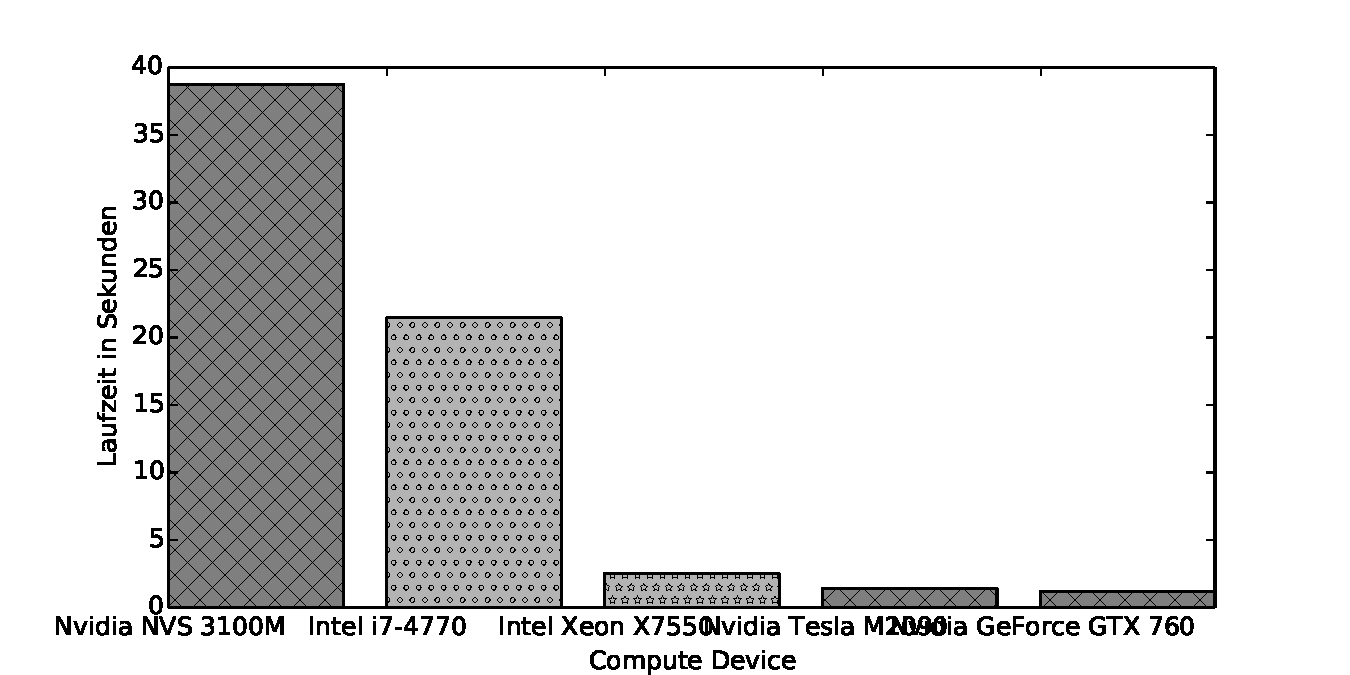
\includegraphics[width=.9\textwidth]{crypto/graphs/speed_comparison_v1.pdf}
	\caption{Performance-Vergleich (TODO danilo: verbessern)}
	\label{img:crypto:speed_comparison_v1}
\end{figure}

TODO: Vergleich inkl. single-threaded

\subsection{Bedeutung f"ur Umgang mit Passw"ortern}

TODO


\printbibliography[heading=subbibliography]
\end{refsection}
